\subsection{Unterbringung der Elektronik}
\label{subsec:Unterbringung_der_Elektronik}

Der grösste Teil der Elektronik befindet sich auf der linken Seite der Maschine unterhalb des Displays gemäss Abbildung \ref{fig:UnterbringungElektronik}. Darin ist einerseits der Motor untergebracht und anderseits das Netzteil, die RFID-Antenne, das Display und das Herz der Maschine - die Hauptplatine. 

\begin{figure}[H]
	\centering
	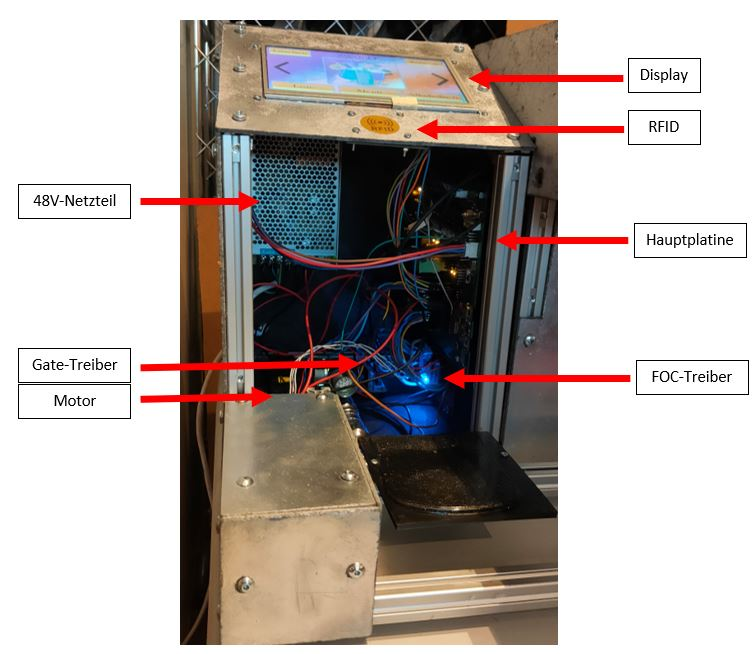
\includegraphics [width=0.8\textwidth]{graphics/UnterbringungElektronik}
	\caption{Unterbringung der Elektronik des Partymixers}
	\label{fig:UnterbringungElektronik}
\end{figure}

Über Kabelkanäle werden die Pumpen und die Durchflussmessgeräte an der Hauptplatine angeschlossen. Diese befinden sich über dem Getränkeschlitten. Um diese an einem X-Profil befestigen zu können wurden auch hier 12 Halterungen gezeichnet und im 3D-Drucker ausgedruckt. Zu sehen ist dies in Abbildung \ref{fig:MontagePumpen}. 

\begin{figure}[H]
	\centering
	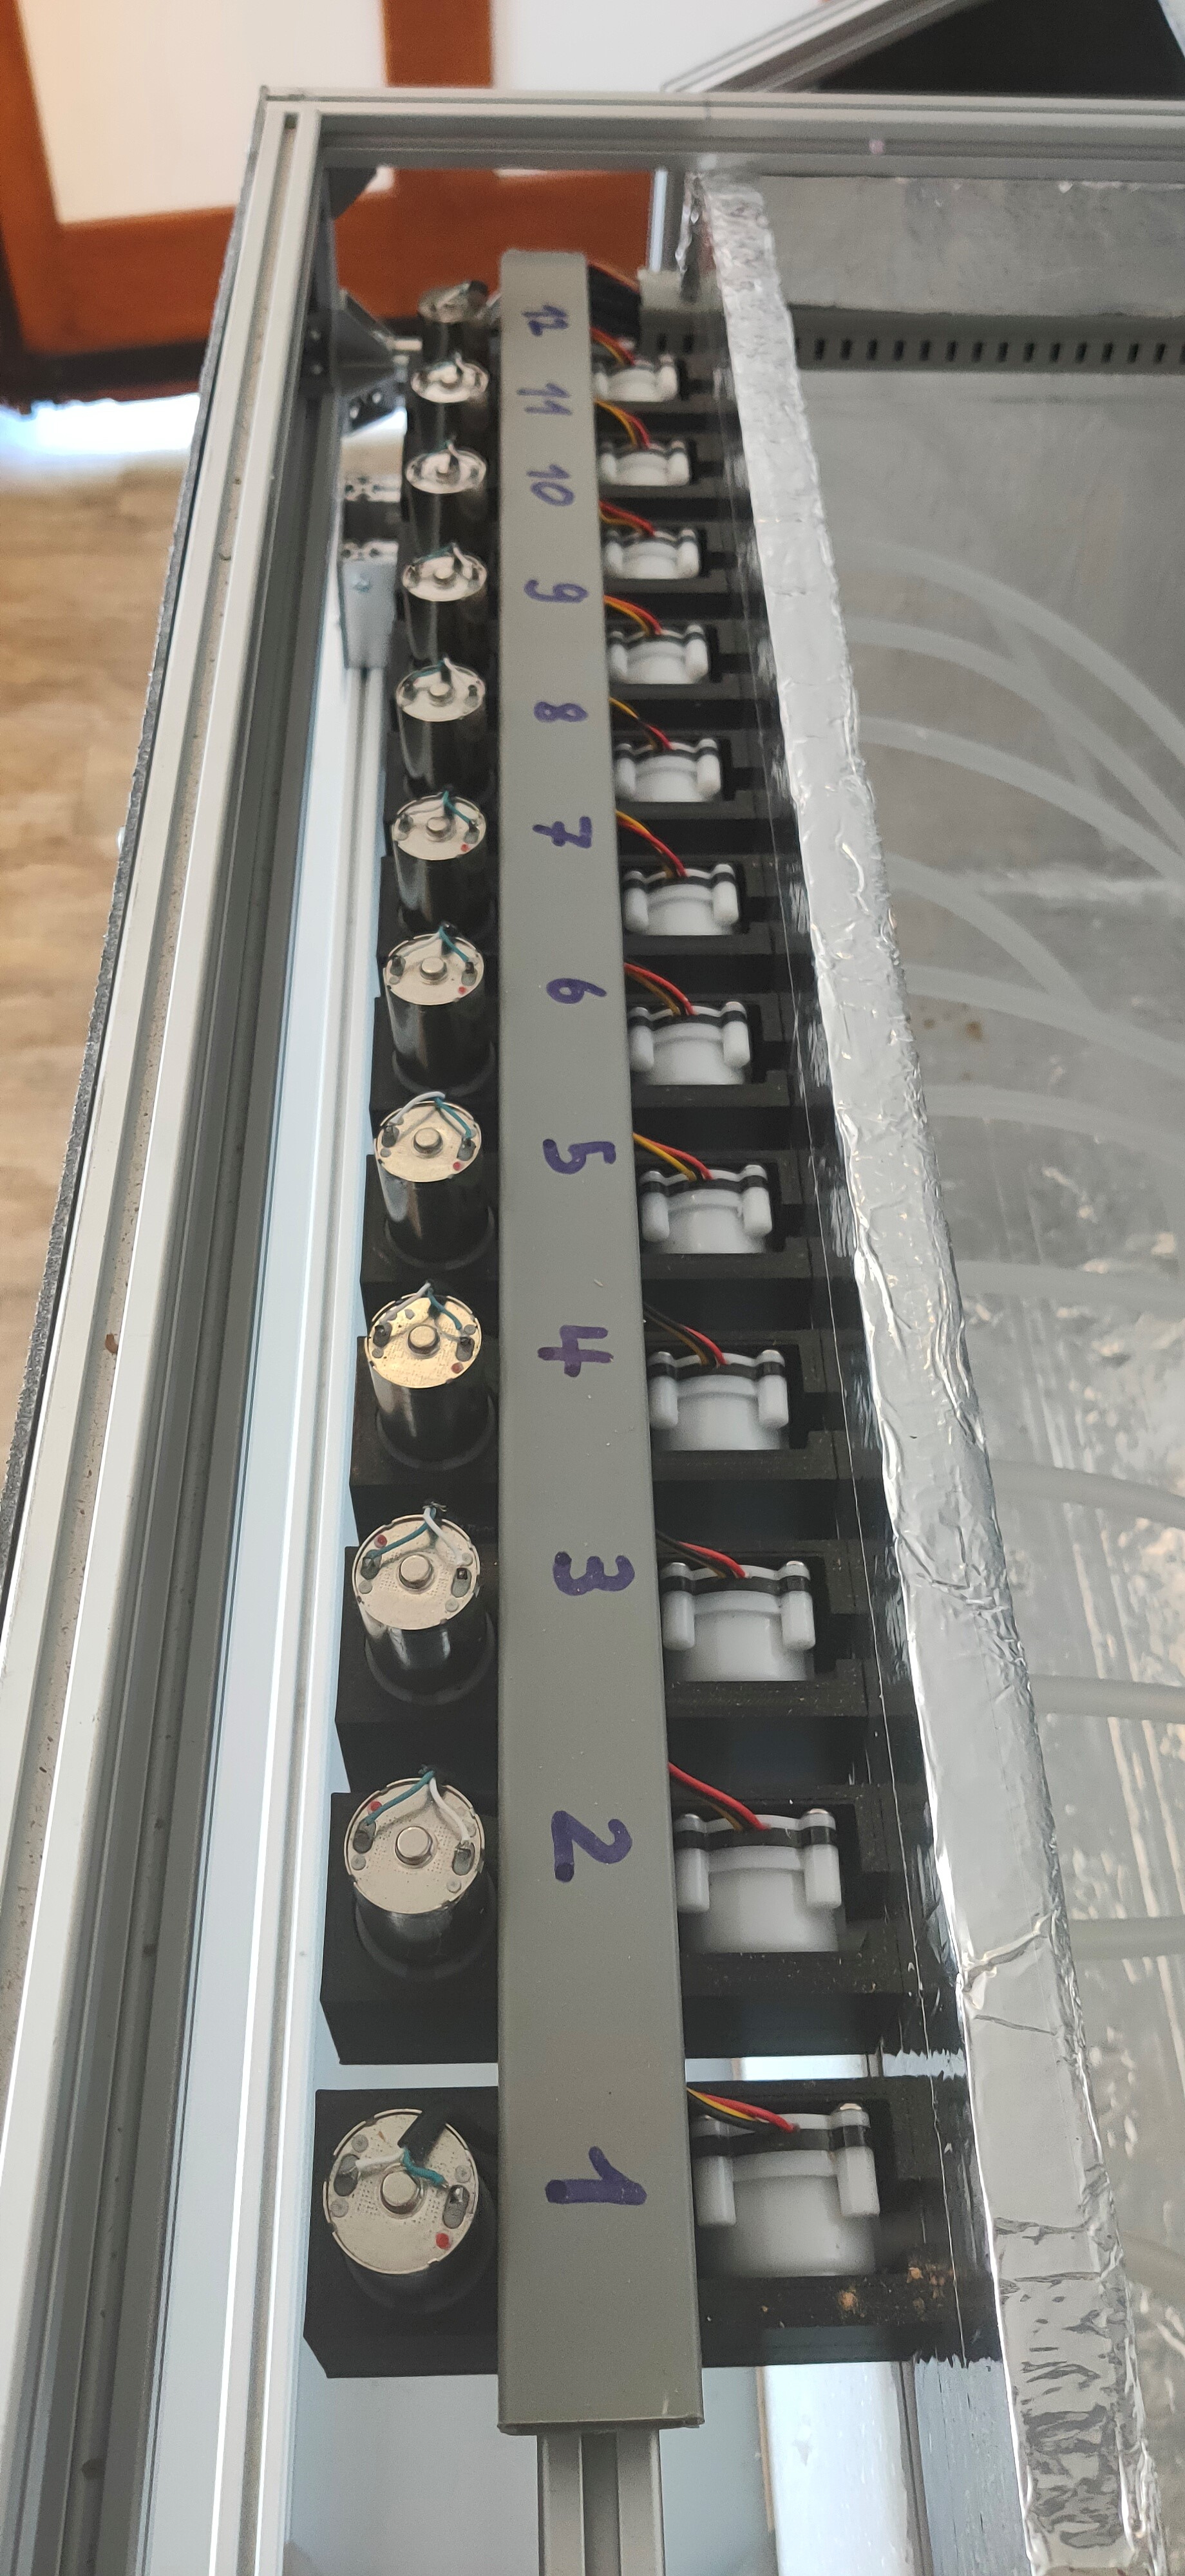
\includegraphics [angle=90, width=0.8\textwidth]{graphics/MontagePumpen}
	\caption{Montage der Pumpen und Durchflussmessgeräte des Partymixers}
	\label{fig:MontagePumpen}
\end{figure}